\section{Two Tower Neural Networks} \label{nn}
A typical Neural Network takes in two inputs, In a two towers neural network used in social media recommendation system, one is an user object and another one is a post object.

\begin{figure}[H]
    \centering
    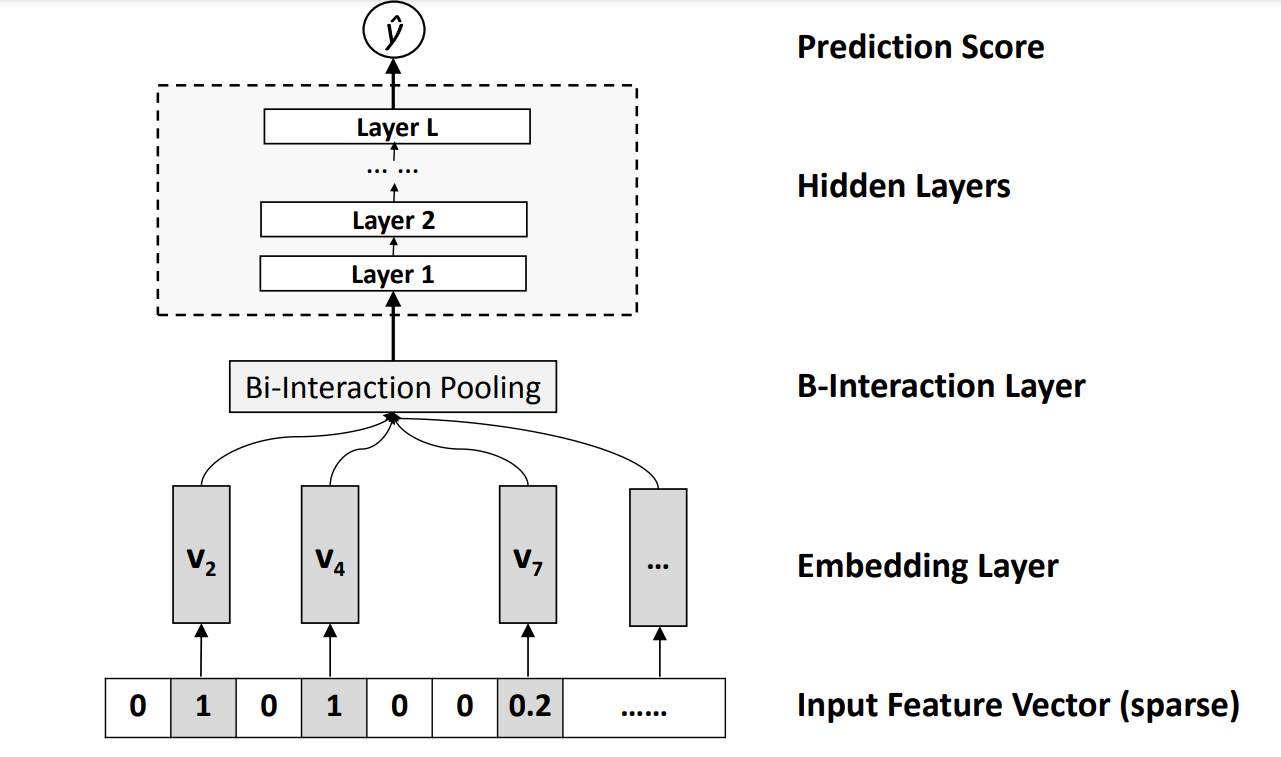
\includegraphics[width=1\linewidth]{Images/single-tower.png}
    \caption{Tower in Two Towers Neural Network \cite{10.1145/3038912.3052569}}
    \label{fig:collaborative-filtering-diagram}
\end{figure}

Above the input layer is the embedding layer; it is a fully
connected layer that projects the sparse representation to
a dense vector.  \cite{10.1145/3038912.3052569} \cite{DBLP:journals/corr/abs-1708-05027} To calculate the output of each tower, we use a neural network. A dot or cosine product is then calculated from the outputs of both neural networks.

\begin{figure}[H]
    \centering
    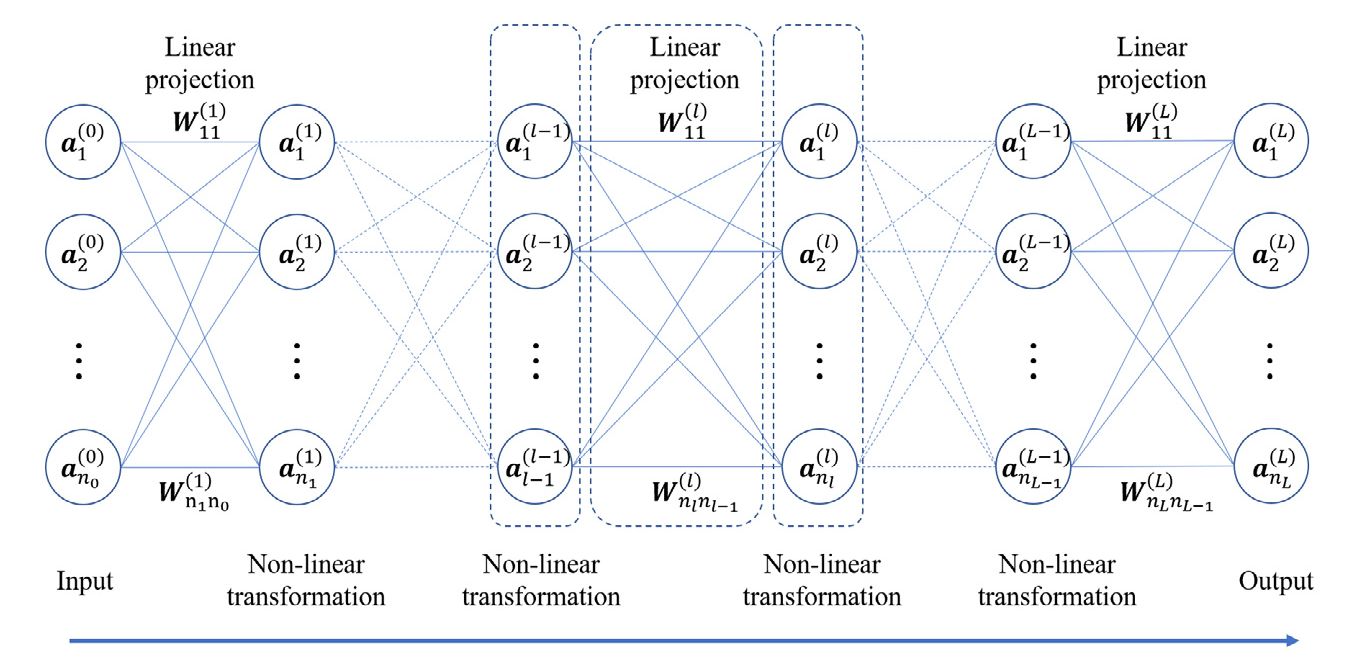
\includegraphics[width=1\linewidth]{Images/neural-network.png}
    \caption{Hidden Layers in A Typical Neural Network \cite{GAO2020409}}
    \label{fig:collaborative-filtering-diagram}
\end{figure}

Between the input and the output of a neural network are layers, each of the layers has a certain amount of neurons. \cite{GAO2020409} The value of the output is calculated from adding weighted values of the previous layer. The same applies for every node of hidden layers. The value of a node $y$ can be calculated with following formula. \cite{9784987} 

\[ y = b + \sum_{i=1}^{n} x_i w_i  \]\

Where $x_i$ is a value previous node and $w_i$ weight associated with it. We calculate sum of weighted values from every single node from previous layer. In the training process some nodes weights will become zero, therefore some nodes can be switched off. Additionally we can introduce a bias $b$ to reduce the error, because it's not affected by the weights. 

\begin{comment}
    $\begin{bmatrix}
    1 & 2 & 3\\
    a & b & c
    \end{bmatrix} $ is a matrix
\end{comment}

\subsection{Embedding}

\subsection{Cold Start}\label{cold-start}

When a new user registers on a social platform, the platform doesn't have any history about the user. Hence, it cannot personalize user's timeline. One option could be to initialize the user vector randomly, or find a similar vector to the most popular ones.

An option for creating embeddings of new posts would be analyzing the content features like the photo, description and hastags.

To improve the precision of recommendation of new items, here are a few proposed algorithms. 

\begin{comment}

aTwo tower neural network architecture 
User embedding
Post embedding
embedding = vector
normalize vector
dot product of post and user vector
pre trained embeddings

\end{comment}

\section{Convolutional Neural Networks}\label{cnn}
Basic Neural Network Concepts apply. \ref{nn} Instead of an input vector, now we have a matrix (an image). Similarly to an elemental neural network, picking a small segment from the input layer, called a filter, creates a point in the next layer. \cite{8609672} This layer is now used as an input for the next layer.

\begin{figure}[H]
    \centering
    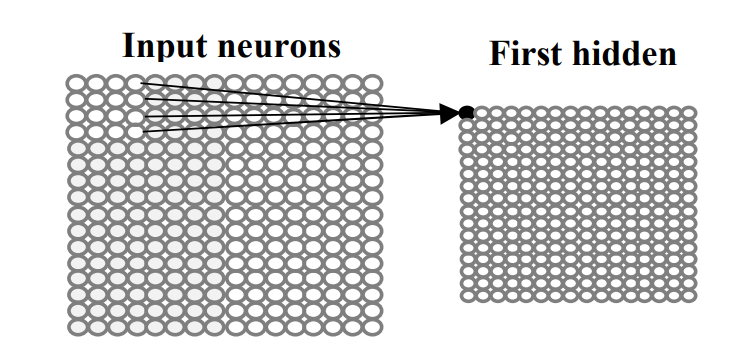
\includegraphics[width=0.5\linewidth]{Images/cnn-layer.png}
    \caption{Basic CNN model with one layer \cite{8609672}}
    \label{fig:collaborative-filtering-diagram}
\end{figure}

The difference between one dimensional neural networks and 2D matrix neural networks is that we can visualise each layer or kernel as an image. Thus we can understand simple convolutional networks better. Some layers are perceived as 3D because of the color depth available.

\begin{figure}[H]
    \centering
    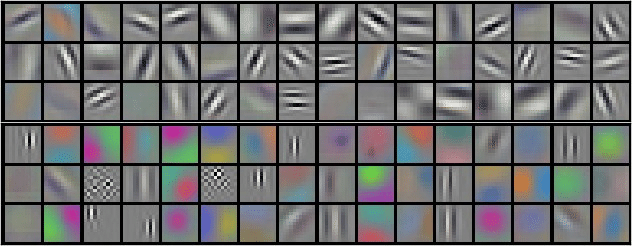
\includegraphics[width=0.5\linewidth]{Images/kernels.png}
    \caption{Kernels learned from AlexNet's first convolutional layer.   \cite{shehata2016using}}
    \label{fig:collaborative-filtering-diagram}
\end{figure}

The final output layer is a vector with probabilities, every value represents propability of the image being classified in a specific class (eg. cat, dog, bird, etc.)



\begin{comment}
\subsection{Alex Net}

\url{https://github.com/amir-saniyan/AlexNet}

\url{https://proceedings.neurips.cc/paper_files/paper/2012/file/c399862d3b9d6b76c8436e924a68c45b-Paper.pdf}

\subsection{VGGNet}

\url{https://github.com/deepblacksky/VGG_tensorflow?tab=readme-ov-file} 

\url{https://arxiv.org/abs/1409.1556}
\subsection{ResNet}

\subsection{GoogLeNet}
GoogLeNet (Inception)

\url{https://github.com/conan7882/GoogLeNet-Inception}

\url{https://research.google/pubs/going-deeper-with-convolutions/}
\subsection{EfficientNet}

\url{https://arxiv.org/abs/1905.11946}

\url{https://github.com/qubvel/efficientnet}
\subsection{Siamese Networks}

\url{https://www.cs.cmu.edu/~rsalakhu/papers/oneshot1.pdf}

\subsection{X (Twitter)}\label{cnn/xalgorithm}

\url{https://github.com/twitter/the-algorithm}

\url{https://blog.x.com/engineering/en_us/topics/open-source/2023/twitter-recommendation-algorithm}

RAPID NET

\end{comment}